\documentclass[]{article}
\title{ECO325: Lecture Notes \\ \small Advanced Economic Theory: Macro}
\author{Tianyu Du}
\date{\today}

\usepackage{spikey}
\usepackage{amsmath}
\usepackage{amssymb}
\usepackage{soul}
\usepackage{float}
\usepackage{graphicx}
\usepackage{hyperref}
\usepackage{xcolor}
\usepackage{chngcntr}

\counterwithin*{equation}{section}


\usepackage[
    type={CC},
    modifier={by-nc},
    version={4.0},
]{doclicense}


\begin{document}
    \maketitle
    \doclicenseThis
    \section*{Notes}
    	\paragraph{Github} \url{https://github.com/TianyuDu/Spikey_UofT_Notes}
    	\paragraph{Color notations}
    		\begin{itemize}
    			\item \textcolor{orange}{Important equations for model setup.}
    			\item \textcolor{blue}{Important equations as results from model.}
    			\item \textcolor{violet}{Implications of model result.}
    		\end{itemize}
    \tableofcontents
    \newpage
    
    \section{Lecture 1. September 6. 2018}
        \begin{definition}
            A \textbf{growth miracle} are episodes where thee growth in a country far exceeds the world average over a extended period of time. \ul{Result} the country experiencing the miracle moves up the wold income distribution.
        \end{definition}
        
        \begin{definition}
            A \textbf{growth disaster} is an episodes where the growth in a country falls short at the world average for an extended period of time. \ul{Result} the country moves down in the world income distribution.
        \end{definition}
    
        \paragraph{Facts} Data from the $20^{th}$ century suggest that
        \begin{enumerate}
            \item Real output grows at a (more or less) constant rate.
            \item Stock of real capital grows at a (more or less) constant rate (but it grows faster than labor input).
            \item Growth rates of real output and the stock of capital are about the same.
            \item The rate of growth of output per capita varies greatly across countries.
        \end{enumerate}
        
        \subsection{Solow Growth Model (continuous time version)}
            \par Solow growth model decomposes the growth in output per capita into portions accounted for by increase in inputs and the portion contributed to increases in productivity.
            \par In the baseline model we denote $K$ as capital, $L$ as labor and $A$ as technology.
            
        \subsubsection{Production Function}
            \begin{remark}
                Harrod-neutral technology here, refer to Uzawa's theorem.
            \end{remark}
            \begin{definition}
                The \textbf{effective labor input} is defined as $A(t)L(t)$
            \end{definition}
            
            \begin{definition}
                The production function is defined as
	            \begin{equation}
                    \textcolor{orange}{Y(t) = F(K(t), A(t)L(t))}
	            \end{equation}
                Typically Cobb-Douglas form is taken
                \[
                    Y(t) = K(t)^\alpha (A(t)L(t))^{1 - \alpha},\ \alpha \in (0, 1)
                \]
            \end{definition}
            
            \begin{property} Properties on production function.
                \begin{enumerate}
                    \item \ul{CRS in $K$ and $AL$}: $Y(cK, cAL) = cY(K, AL),\ \forall c \geq 0$ implies
                        \begin{itemize}
                            \item All gains from specialization have been exhausted.
                            \item Inputs other than $K$ and $AL$ are unimportant.
                        \end{itemize}
                \end{enumerate}
            \end{property}
            
            \begin{definition}
                Define $c := \frac{1}{AL}$, the \textbf{intensive form} of production function is
                \[
                    y(t) = \frac{Y(t)}{A(t)L(t)} = f(k(t))
                \]
                where $y := \frac{Y}{AL}$ denotes the \textbf{output per unit of effective labor} and $k := \frac{K}{AL}$ denote the capital stock per unit of effective labor.
            \end{definition}
	
	\section{Lecture 2 September 13. 2018}
		\subsection{Solow Growth Model: Setup}
			\begin{definition}
				\textbf{Production function} $F: \R^2_{+} \rightarrow \R_+$ maps input factors:
				\begin{itemize}
					\item $K(t) := $ aggregate capital stock at time $t$.
					\item $L(t) := $ aggregate labor supple at time $t$.
					\item $A(t) := $ labor argument technology (\ul{effectiveness of labor}) at time $t$.
				\end{itemize} 
				to output values ($Y(t) := $ aggregate output at time $t$.) The production function takes the form of
				\[
					Y(t) = F(K(t), A(t)L(t))
				\]
			\end{definition}
			
			\begin{assumption}[Assumptions on Production Function]
				The production function are assumed to satisfy the following assumptions: 
				\begin{itemize}
					\item \ul{Constant Return to Scale}: \[cF(K(t), A(t)L(t)) = F(cK(t), cA(t)L(t)),\ \forall c > 0\]
				\end{itemize}
			\end{assumption}
			
			\begin{definition}
				The \textbf{intensive form of production function} is defined as the output per effective unit of labor. Let $f(t) := \frac{Y(t)}{A(t)L(t)}$ and $k(t) := \frac{K(t)}{A(t)L(t)}$ be the output and capital per unit of effective labor respectively. By the assumption of \emph{CRS} on \emph{aggregate} production function, take $c = \frac{1}{A(t)L(t)}$. The \emph{intensive form} production function can be expressed as
				\begin{equation}
					\textcolor{orange}{
						y(t) = f(k(t))
					}
				\end{equation}
			\end{definition}
			
			\begin{assumption}[Assumptions on Intensive Form Production Function] the function $f(\cdot): \R_+ \rightarrow \R_+$ is assumed to satisfy \emph{Inada Conditions}.
				\begin{enumerate}
					\item $f(0) = 0$: capital is necessary for production.
					\item $f'(k) > 0,\ \forall k \in \R_+$: the marginal return of capital per effective unit of labor is positive.
					\item $f''(k) < 0,\ \forall k \in \R_+$: capital per effective unit of labor is experiencing diminishing marginal return.
					\item $\lim_{k \to 0}f'(k) = \infty$
					\item $\lim_{k \to \infty}f''(k) = 0$
				\end{enumerate}
				\emph{The role of above conditions is to ensure that the path of the economy does not diverge.}
			\end{assumption}
			
			\begin{example}[Cobb-Douglas Production Function]
				Consider the Cobb-Douglas production function
				\[
					Y(t) = K(t)^\alpha (A(t)L(t))^{1 - \alpha},\ \alpha \in (0, 1)
				\]
				
				\begin{proof}[Check]
					Let $c \in \R_+$, 
					\begin{gather*}
						F(cK, cAL) = (cK)^\alpha (cAL)^{1 - \alpha} \\
						= c^\alpha c^{1-\alpha} K^\alpha AL^{1-\alpha} \\
						= cK^{\alpha} AL^{1-\alpha} = cF(K, AL)
					\end{gather*}
					CRS on aggregate form is shown. \\
					Notice that $f(k) = k^{\alpha}$ \\
					And 
					\begin{enumerate}
						\item $f(0) = 0^{\alpha} = 0$
						\item $f'(k) = \alpha k ^ {\alpha - 1} > 0, \forall k \in \R_+$
						\item $f''(k) = (\alpha - 1)\alpha k ^ {\alpha - 2} < 0, \ \forall k \in \R_+$
						\item $\lim_{k \to 0} \alpha \frac{1}{k^{1-\alpha}} = \infty$
						\item $\lim_{k \to \infty} \alpha \frac{1}{k^{1-\alpha}} = 0$
					\end{enumerate}
					Inada conditions on intensive form are shown. \\
				\end{proof}
			\end{example}
			
			\begin{assumption}[Assumptions on the Economy]
				Assume the initial values of $K, A, L$ are given and strictly positive. Labor and Knowledge are assumed to grow at an exogenously given constant rate, denoted as $n, g$ respective.
				\begin{gather}
				\textcolor{orange}{
					\dot{L(t)} = nL(t),\ n > 0 }\\
					\textcolor{orange}{
						\dot{A(t)} = gA(t),\ g > 0
					}
				\end{gather}
			\end{assumption}
			
			\begin{proposition}
				Notice the \ul{growth rate} of variable $X$ is given by 
				\[
					g_X := \frac{\dot{X(t)}}{X(t)} = \pd{\ln{X(t)}}{t}
				\]
			\end{proposition}
			\begin{proof}
				\begin{gather*}
					\pd{\ln{X(t)}}{t} = \pd{\ln{X(t)}}{X(t)} \pd{X(t)}{t} \\
					= \frac{1}{X(t)} \dot{X(t)}
					= \frac{\dot{X(t)}}{X(t)}
					= g_X \\
				\end{gather*}
			\end{proof}
			
			\begin{proposition}
				The functional form of technology and labor at time $t$ can be found by solving ODEs 
				\begin{gather}
					\textcolor{orange}{
						L(t) = e^{nt} L(0)
						} \\
					\textcolor{orange}{
						A(t) = e^{gt} A(0)
						}
				\end{gather}
			\end{proposition}
			
			\par Assume there is \emph{no government} and the Solow economy is a \emph{closed economy}. The output is divided between \emph{consumption} and \emph{investment} as 
			\[
				Y(t) = C(t) + I(t)
			\]
			And given $\delta$ as depreciation rate of capital, in discrete time (let $\Delta t = 1$)we have 
			\begin{gather*}
				K(t+1) = (1-\delta)K(t) + I(t) \\
				\iff I(t) = K(t+1) - K(t) + \delta K(t) \\
				\tx{As } \Delta \to 0 \tx{ (convert to continuous time)}\\
				I(t) = \dot{K}(t) + \delta K(t)
			\end{gather*}
			
			\begin{assumption}
				Assume investment equals saving and a constant friction $s \in [0, 1]$ of output is saved at each epoch. The marginal propensity to save, $s$ is given exogenously.
			\end{assumption}
			
			\par Therefore,
			\begin{gather*}
				I(t) = sY(t) \implies \dot{K}(t) + \delta K(t) = sY(t) \\
				\implies \textcolor{orange}{
					\dot{K}(t) = sY(t) - \delta(K(t))
					}
			\end{gather*}
			
			\subsection{Dynamics of $k(t)$}
				\par For simplicity, assuming $n, g, \delta > 0$ and the dynamics of capital per effective unit of labor follows: 
				\begin{gather*}
					\dot{k}(t) := \pd{k(t)}{t} = \pd{}{t} \frac{K(t)}{A(t)L(t)} \\
					= \frac{\dot{K}AL - K(\dot{A}L + A\dot{L})}{(AL)^2} \\
					= \frac{\dot{K}}{AL} - \frac{K\dot{A}L}{(AL)^2} - \frac{K A\dot{L}}{(AL)^2} \\
					= \frac{sY - \delta K}{AL} - \frac{\dot{A}}{A}\frac{K}{AL} - \frac{\dot{L}}{L} \frac{K}{AL} \\
					= sy(t) - (n + g + \delta) k(t)
				\end{gather*}
				Where $s y(t)$ is the \textbf{actual investment} per unit effective unit of labor and $(n + g + \delta) k(t)$ is the \textbf{break-even investment} per effective unit of labor.
				
			\begin{remark}
				The \ul{convergence speed} is \ul{inversely} correlated with the value of $|| k(t) - k^* ||$, where $k^*$ denotes the steady state level of capital stock per effective unit of labor.
			\end{remark}
			
			\begin{remark}
				With \ul{convex} production function ($f''(k) > 0$), then $k(t) < k^* \implies \dot{k} < 0$ and $k(t) > k^* \implies \dot{k} > 0$. The steady state value $k^*$ is \ul{steady but not stable} (with $k(t) \neq k^*$, $k$ does not automatically converge to $k^*$).
			\end{remark}
	
	\section{Lecture 3 September 20. 2018}
		\subsection{Dynamic Transitions}
			\begin{remark}
				For the dynamic transition function of capital per unit of effective labor:
				\begin{equation}
				\textcolor{orange}{
					\dot{k}(t) = sf(k(t)) - (n+g+\delta)k(t)
					}
				\end{equation}
			\end{remark}
			\paragraph{} And dynamic transition and phase diagram can be expressed as
			\begin{figure}[h]
				\centering
				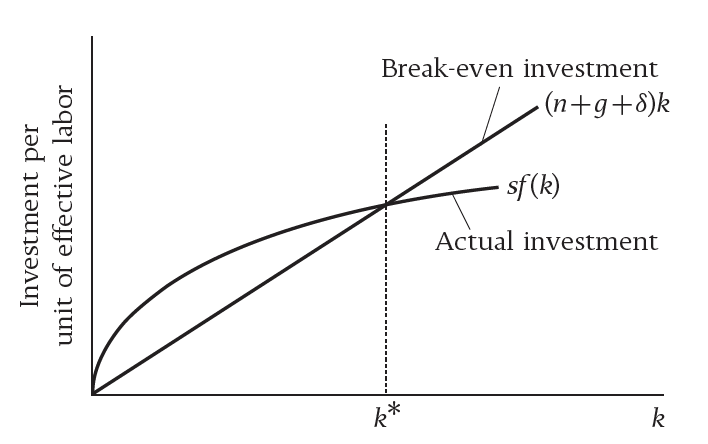
\includegraphics[width=0.6\linewidth]{figures/3_1.png}
				\caption{Dynamic Transition of Capital Per Unit of Effective Labor}
			\end{figure}
			
			\begin{figure}[h]
				\centering
				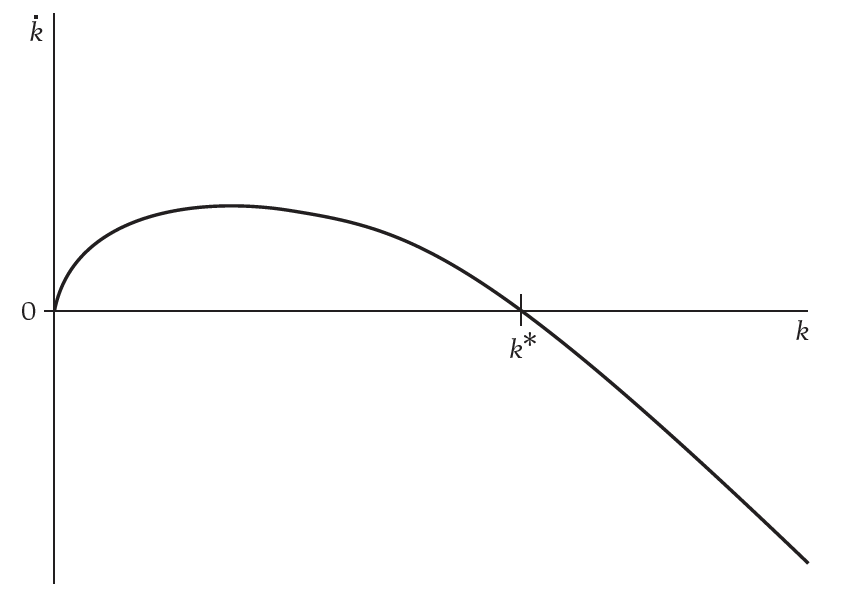
\includegraphics[width=0.6\linewidth]{figures/3_2.png}
				\caption{Phase Diagram of Capital Per Unit of Effective Labor}
			\end{figure}
			
			\begin{definition}
			\textbf{Steady level of capital per unit of effective labor($k^*$)} is defined as the level of capital per unit of effective labor that equates break-even investment per unit of effective labor and actual investment per unit of effective labor. \footnote{The definition can also be expressed as $k^* := \{k \in \R_{+}: \hat{k} = 0\}$}
				\[
					k^* := \{k \in \R_{+}: sf(k) = (n+g+\delta) k\}
				\]
			\end{definition}
			
			\begin{remark}
				The values of other endogenous variables at steady state are also derived from $k^*$.
				\begin{example}
					\begin{gather}
						y^* = f(k^*) \\
						i^* = sf(k^*) = (n+g+\delta) k^* \\
						c^* = y^* - i^* = f(k^*) - (n+g+\delta)k^* = (1-s)f(k^*)
					\end{gather}
				\end{example}
				For the growth rate of each endogenous variable (per unit of effective labor). 
					\begin{gather}
						\pd{k(t)}{t}|_{k=k^*} = 0 \\
						\pd{c(t)}{t}|_{k=k^*} = 0 \\
						\pd{y(t)}{t}|_{k=k^*} = 0 
					\end{gather}
					above relations are equivalent to 
					\begin{gather}
						\tx{On steady state} \begin{cases}
							\dot{c}(t) = 0 \\
							\dot{k}(t) = 0 \\
							\dot{y}(t) = 0 \\
						\end{cases}
					\end{gather}
			\end{remark}
			
			\begin{proof}
				By definition of consumption per unit of effective labor,\\
				$c(\cdot) = (1-s)f(k(t))$ \\
				$\implies \dot{c}(t) := \pd{c(\cdot)}{t} = (1-s)f'(k(t)) \dot{k(t)}$ by chain rule \\
				Since $\dot{k}|_{k=k^*} = 0$ and $(1-s)f'(k(t)) < \infty$ \\
				Thus $\dot{c}(t)|_{k=k^*} = 0$
			\end{proof}
			
		\subsection{Balanced Growth Path}
			\begin{definition}
				A \textbf{balanced growth path} is a situation where each variable in the model are all growing at a constant rate. \footnote{Variables are not required to grow at the same rate by this definition.} \footnote{Variables remaining fixed are also considered as growing at a constant rate ($g=0$).}
			\end{definition}
			
			\subsubsection{Growth Rates on Balanced Growth Path}
			\paragraph{Population and Technology} By definition of population and technological progress,
			\begin{gather}
				g_A := \frac{\dot{A}}{A} = g \\
				g_L := \frac{\dot{L}}{L} = n
			\end{gather}
			
			\paragraph{Capital per person} Since $\frac{K(t)}{L(t)} = \frac{k(t)A(t)L(t)}{L(t)} = k(t)A(t)$, and the growth rate of $x(t)$ can be found as $\pd{\ln{x(t)}}{t}$. Then
			\begin{proof}[Solution]
				\begin{gather*}
					\pd{\ln{\frac{K(t)}{L(t)}}}{t} = \pd{k(t)A(t)}{t} \\
					= \pd{\ln{k(t)}}{t} + \pd{\ln{A(t)}}{t} \\
					= \frac{\dot{k}(t)}{k(t)} + g \\
				\end{gather*}
				And at the steady state, by definition, $\dot{k}(t)|_{k-k^*} = 0$, therefore 
				\begin{equation}
					\textcolor{blue}{
						g_{\frac{K}{L}}^* = g
					}
				\end{equation}
			\end{proof}
			
			\paragraph{Output and Consumption per person} Similarly,
			\begin{proof}[Solution]
				\begin{gather*}
					\frac{Y(t)}{L(t)} = y(t)A(t) \\
					g_{\frac{Y}{L}} = \pd{\ln{y(t)} + \ln{A(t)}}{t} \\
					= \pd{\ln{y}}{t} + \pd{\ln{A(t)}}{t} \\
					= g + \frac{\dot{y}}{y}
				\end{gather*}
				and for consumption per person,
				\begin{gather*}
					\frac{C(t)}{L(t)} = c(t)A(t)\\
					g_{\frac{C}{L}} = g + \frac{\dot{c}}{c} \\
				\end{gather*}
				Thus, on the balanced growth path, \footnote{$g_X^*$ denotes the growth rate of variable $X$ on the balanced growth path.}
				\begin{gather}
					\textcolor{blue}{
						g_{\frac{Y}{L}}^* = g
					}
					\\
					\textcolor{blue}{
						g_{\frac{C}{L}}^* = g
					}
				\end{gather}
			\end{proof}
			
			\begin{proposition}
				Along the balanced growth path, consumption and output per person also growth at rate $g$.
			\end{proposition}
			
			\begin{proposition}
				Along the balanced growth path, aggregate variables, $Y(t), I(t), C(t)$ are all growing at a rate $n + g$.
				\begin{equation}
					\textcolor{blue}{
						g_{Y}^* = g_{C}^* = g_{I}^* = n + g
						}
				\end{equation}
			\end{proposition}
			\begin{proof}
				\begin{gather*}
				g_{K} = \pd{\ln{K(t)}}{t} \\
				= \pd{\ln{A(t)L(t)k(t)}}{t} \\
				= \pd{\ln{A(t)}}{t} + \pd{\ln{L(t)}}{t} + \pd{\ln{k(t)}}{t} \\
				= g + n + \frac{\dot{k}}{k}
				\end{gather*}
				and at balanced growth path, $\frac{\dot{k}}{k}|_{k=k^*} = 0$, therefore 
				\begin{equation}
					\textcolor{blue}{
						g_K^* = n + g
					}
				\end{equation}
				and proof for $C(t)$ and $I(t)$ follows the same path.
			\end{proof}
		
		\begin{definition}
			The \textbf{golden rule level of capital per unit of effective labor} ($k_G$) is the \ul{steady state level of} capital per unit of effective labor that maximizes steady state consumption per unit of effective labor.
				\[
					k_G = argmax_{k^* \in \textbf{k}^*(\Theta)} \{c^* = f(k^*) - (n+g+ \delta) k^*\}
				\]
		\end{definition}
		
		\begin{proof}[First Order Necessary Condition]
		Solve \\
			\begin{gather*}
				\pd{c^*(k^*)}{k^*} = 0 \\
				\implies \pd{f(k^*) - (n+g+\delta)k^*}{k^*} = 0 \\
				\implies f'(k^*) = (n+g+\delta)
			\end{gather*}
			Thus, golden rule level of capital stock per unit of effective labor $k_G$ can be expressed as \footnote{Notice that the zero solution, $k^* = 0$ is a trivial steady state and we ignore this case during this course.}
			\begin{equation}
				k_G = \{k \in \R_{+}: f'(k) = (n+g+\delta)\}
			\end{equation}
		\end{proof}
		
		\subsection{Experiment}
			\subsubsection{Impact of Change in the Saving Rate ($s_1 > s_0$)}
			\paragraph{} Suppose at time $t_0$, the saving rate parameter increases discretely: $s_0 \rightarrow s_1$.
			\begin{figure}
				\centering
				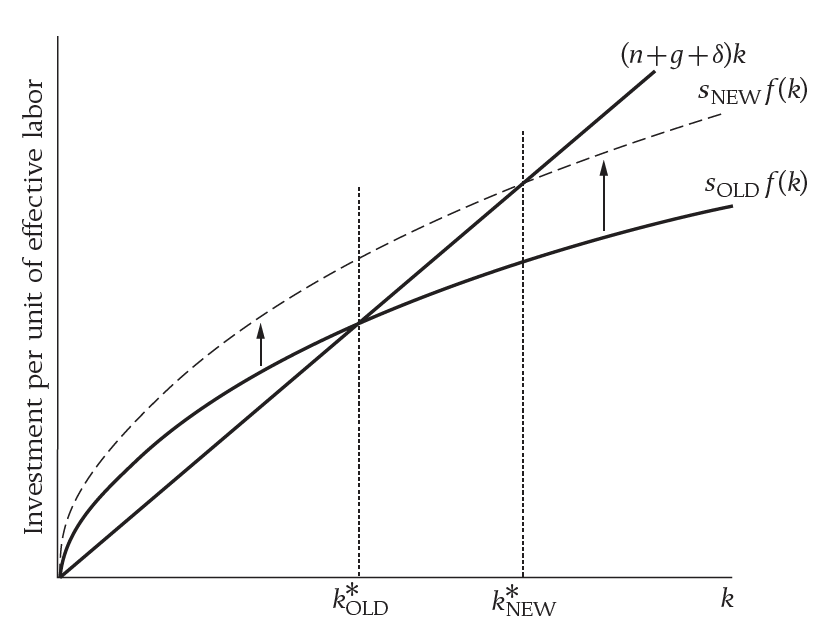
\includegraphics[width=0.5\linewidth]{figures/3_3.png}
				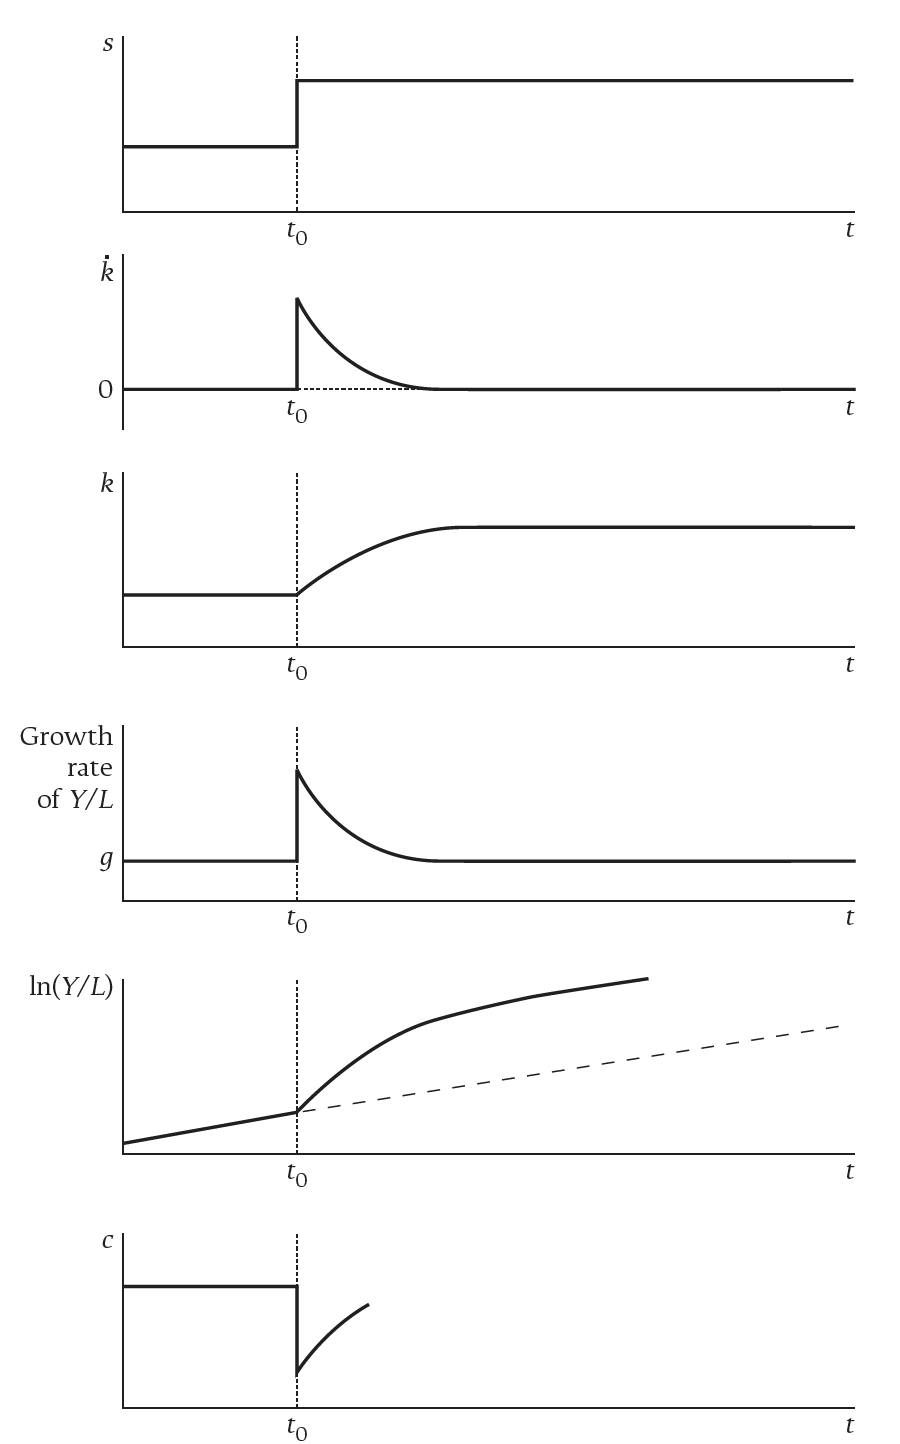
\includegraphics[width=0.5\linewidth]{figures/3_4.png}
				\caption{Effect of an Increase in Saving Rate.}
			\end{figure}
			
			\begin{remark}
				The relation of $c_0^*$ and $c_1^*$ depends on the relative position of $s_1$ and the golden rule level of saving rate $s_G$.
			\end{remark}
			
			\subsubsection{Derive the Effect of Change in $s$ Mathematically}
				\paragraph{Goal} Find $\pd{k^*}{s}$. And notice that $k^*(n+g+\delta) = sf(k^*)$ for any steady state capital level $k^*$. And the steady state level of capital per unit of effective labor can be written as a function of parameters, as $k^*(n, g, \delta, s)$.
				
			\paragraph{Impact on $k^*$}
			\begin{proof}[Solution]
				At any steady state level, $k^*$ satisfies \\
				\[sf(k^*(n,g,\delta,s)) = (n+g+\delta)k^*(n,g,\delta,s)\] \\
				Differentiate both sides with respect to $s$, \\
				We have \[sf'(k^*)\pd{k^*}{s} + f(k^*) = (n+g+\delta)\pd{k^*}{s}\] \\
				Rearrange and get \\
				\[
					\pd{k^*}{s} = \frac{f(k^*)}{(n+g+\delta) - sf'(k^*)}
				\] \\
				Notice that the slope of break-even investment is greater than the slope of the actual investment at the steady state, therefore \[\pd{k^*}{s} > 0\] \\
			\end{proof}
			
			\paragraph{Impact on $y^*$}
			\begin{proof}[Solution]
				Using chain rule we have
				\begin{gather*}
					\pd{y^*}{s} = \pd{f(k^*)}{s} \\
					= \pd{f(k^*)}{k^*} \pd{k^*}{s} > 0,\ \forall k^* \in \textbf{k}^*({\Theta})
				\end{gather*}
			\end{proof}
			
			\par To get a sense on how much $y^*$ changes wit respect to change in $s$, we could look at the \ul{elasticity}.
			\[
				\eta = \pd{y^*}{s}\frac{s}{y^*} = f'(k^*) \pd{k^*}{s} \frac{s}{f(k^*)} = \frac{f'(k^*)s}{(n+g+\delta) - sf'(k^*)}
			\]
			Recall that $(n+g+\delta) = \frac{sf(k^*)}{k^*}$ and rearrange the elasticity
			\begin{gather*}
				\eta = \pd{y^*}{s}\frac{s}{y^*} \\
				= \frac{f'(k^*)s}{(n+g+\delta) - sf'(k^*)} \\
				= \frac{s f'(k^*)}{\frac{s f(k^*)}{k^*} - sf'(k^*)} \\
				= \frac{f'(k^*)}{\frac{f(k^*)}{k^*} - f'(k^*)} \\
				= \frac{f'(k^*) \frac{k^*}{f(k^*)}}{1 - f'(k^*)\frac{k^*}{f(k^*)}} \\
				= \textcolor{blue}{
					\frac{\alpha_K}{1 - \alpha_K}
					} \\
			\end{gather*}
			
			\begin{remark}
				$\alpha_K$ denotes the elasticity of output per unit of effective unit labor with respect to capital stock per unit of effective labor, along the balanced growth path. And
				\[
					\alpha_K \approx \frac{1}{3}
				\]
			\end{remark}
			
			\begin{remark}
				If the production function is in the Cobb-Douglas form, then $\alpha_K = \alpha$.
			\end{remark}
			
			\begin{example}
				If $\alpha_K \approx \frac{1}{3}$ then $\pd{y^*}{s}{s}{y^*} \approx \frac{1}{2}$.
			\end{example}
			
			\paragraph{Impact on $c^*$} Notice that on the balanced growth path $c^* = y^* - i^*$.
			\begin{equation}
				c^* = f(k^*) - (n+g+\delta)k^*
			\end{equation}
			and differentiate with respect to $s$
			\[
				\pd{c^*}{s} = [f'(k^*) - (n+g+\delta)] \pd{k^*}{s}
			\]
			And notice that the sign of $\pd{c^*}{s}$ depends on the relative slope of production function and break-even investment.
			By the first order condition of golden rule level of capital per unit of effective labor, $(n+g+\delta) = f'(k_G)$
			\begin{gather*}
				\pd{c^*}{s} = [f'(k^*) - f'(k_G)]\pd{k^*}{s}
			\end{gather*}
			And 
			\begin{equation*}
				\begin{cases}
					k^* = k_G \implies f'(k^*) = f'(k_G) \implies \pd{c^*}{s} = 0 \\
					k^* < k_G \implies f'(k^*) > f'(k_G) \implies \pd{c^*}{s} > 0 \\
					k^* > k_G \implies f'(k^*) < f'(k_G) \implies \pd{c^*}{s} < 0
				\end{cases}
			\end{equation*}
\end{document}








